\section*{Приложение. Безынерционная модель}\label{sect:bezinerz}

На протяжении всей работы делаются ссылки на модель экипажа с омни-колесами, широко представленную в литературе (например, в \cite{Borisov2011, formalskii, ZobovaTatarinovPMM}). Для полноты изложения, опишем здесь эту модель и приведем ее уравнения движения.

В данной модели омниколеса рассматриваются в предположении, что массой и инерцией роликов можно пренебречь. Поэтому будем называть эту модель безынерционной. На систему налагаются неголономные связи, ограничивающие направление скорости скольжения в точках контакта колес с опорной поверхностью, на которой стоит экипаж. Сила трения в контакте не вводится, т.е. скольжение дисков колес считается идеальным.
% Эти идеализированные модели имеют существенно меньше степеней свободы, чем ``реальный'' омниэкипаж, и легче поддаются аналитическому исследованию.

Приведем в качестве примера уравнения движения, полученные в работе \cite{Borisov2011}. Авторы принимают простейшую модель омниколеса как плоского диска, для которого скорость точки контакта с опорной поверхностью направлена вдоль прямой, составляющей некоторый угол $\psi$ с плоскостью колеса (см. рис.~\ref{fig:bor_wheel_scheme}). Связь, наложенная на колесо в таком случае имеет вид
$$
    \vec{v_C} \cdot \vec{i} = 0,
$$
где $\vec{v_C}$ -- скорость точки контакта $C$, $\vec{i}$ -- единичный вектор, направленный вдоль ``оси ролика'' на колесе с номером $i$. Хотя сами тела роликов исключены из рассмотрения, эффекты от их кинематики все же моделируются данными связями.\\

\begin{figure}[ht!]
    \centering
    % 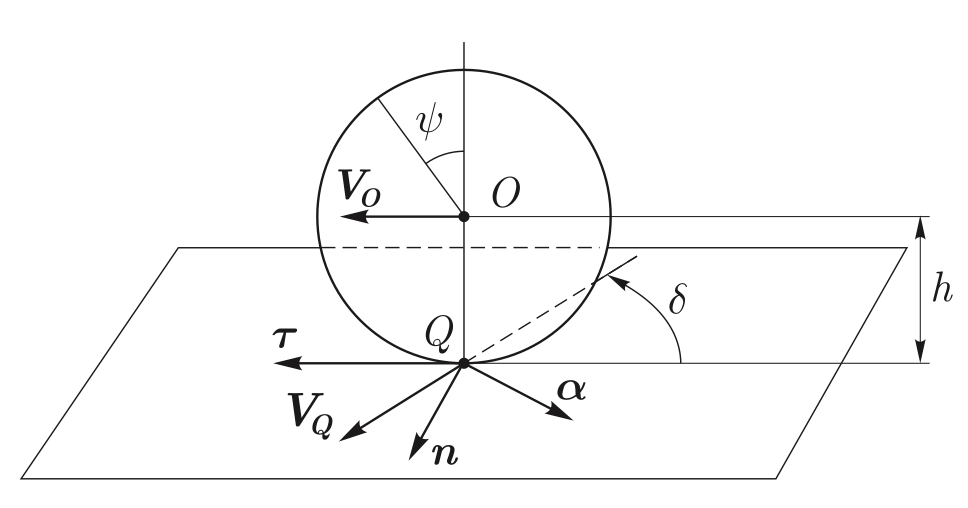
\includegraphics[width=0.75\textwidth]{content/parts/3_friction/diploma/img/art/bor_wheel_scheme.png}
    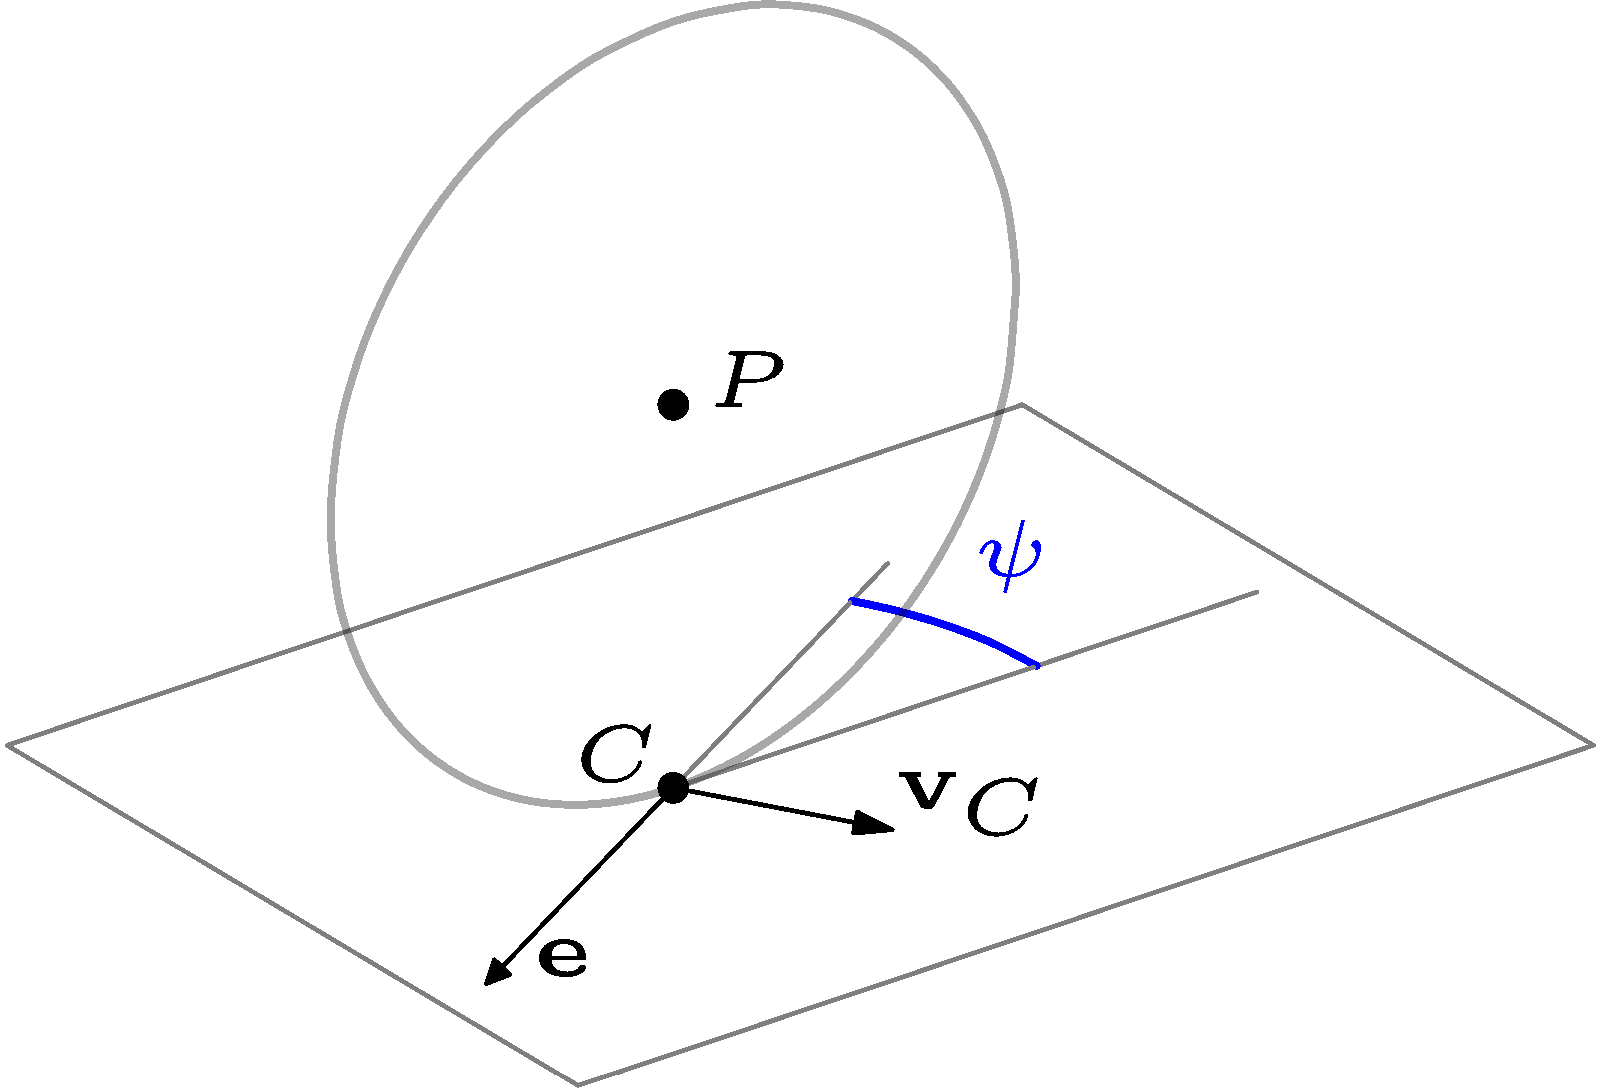
\includegraphics[width=0.5\textwidth]{content/pic/asy/wheel_bor.png}
    % \asyinclude[width=0.75\textwidth]{content/pic/asy/wheel_bor.asy}
    \caption{Безынерционная модель колеса}
    \label{fig:bor_wheel_scheme}
\end{figure}

Авторы \cite{Borisov2011} получают уравнения движения для экипажа с произвольным количеством и расположением колес, закрепленных так, что их оси неподвижны относительно платформы, а оси роликов повернуты на произвольные углы относительно плоскостей соответствующих колес (см. фиг.~\ref{fig:bor_vehicle}).

\begin{figure}[ht!]
    \centering
    % 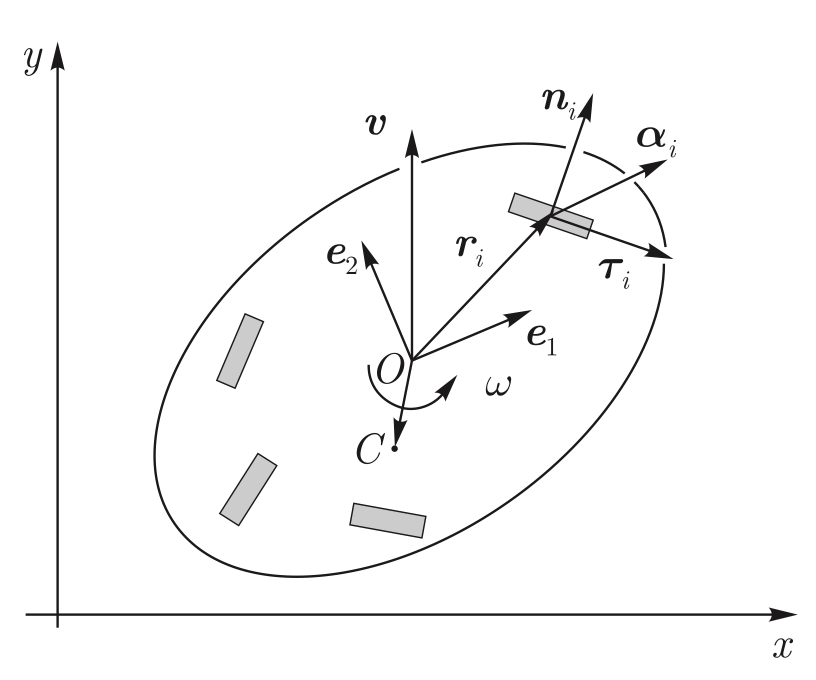
\includegraphics[width=0.75\textwidth]{content/parts/3_friction/diploma/img/art/bor_vehicle.png}
    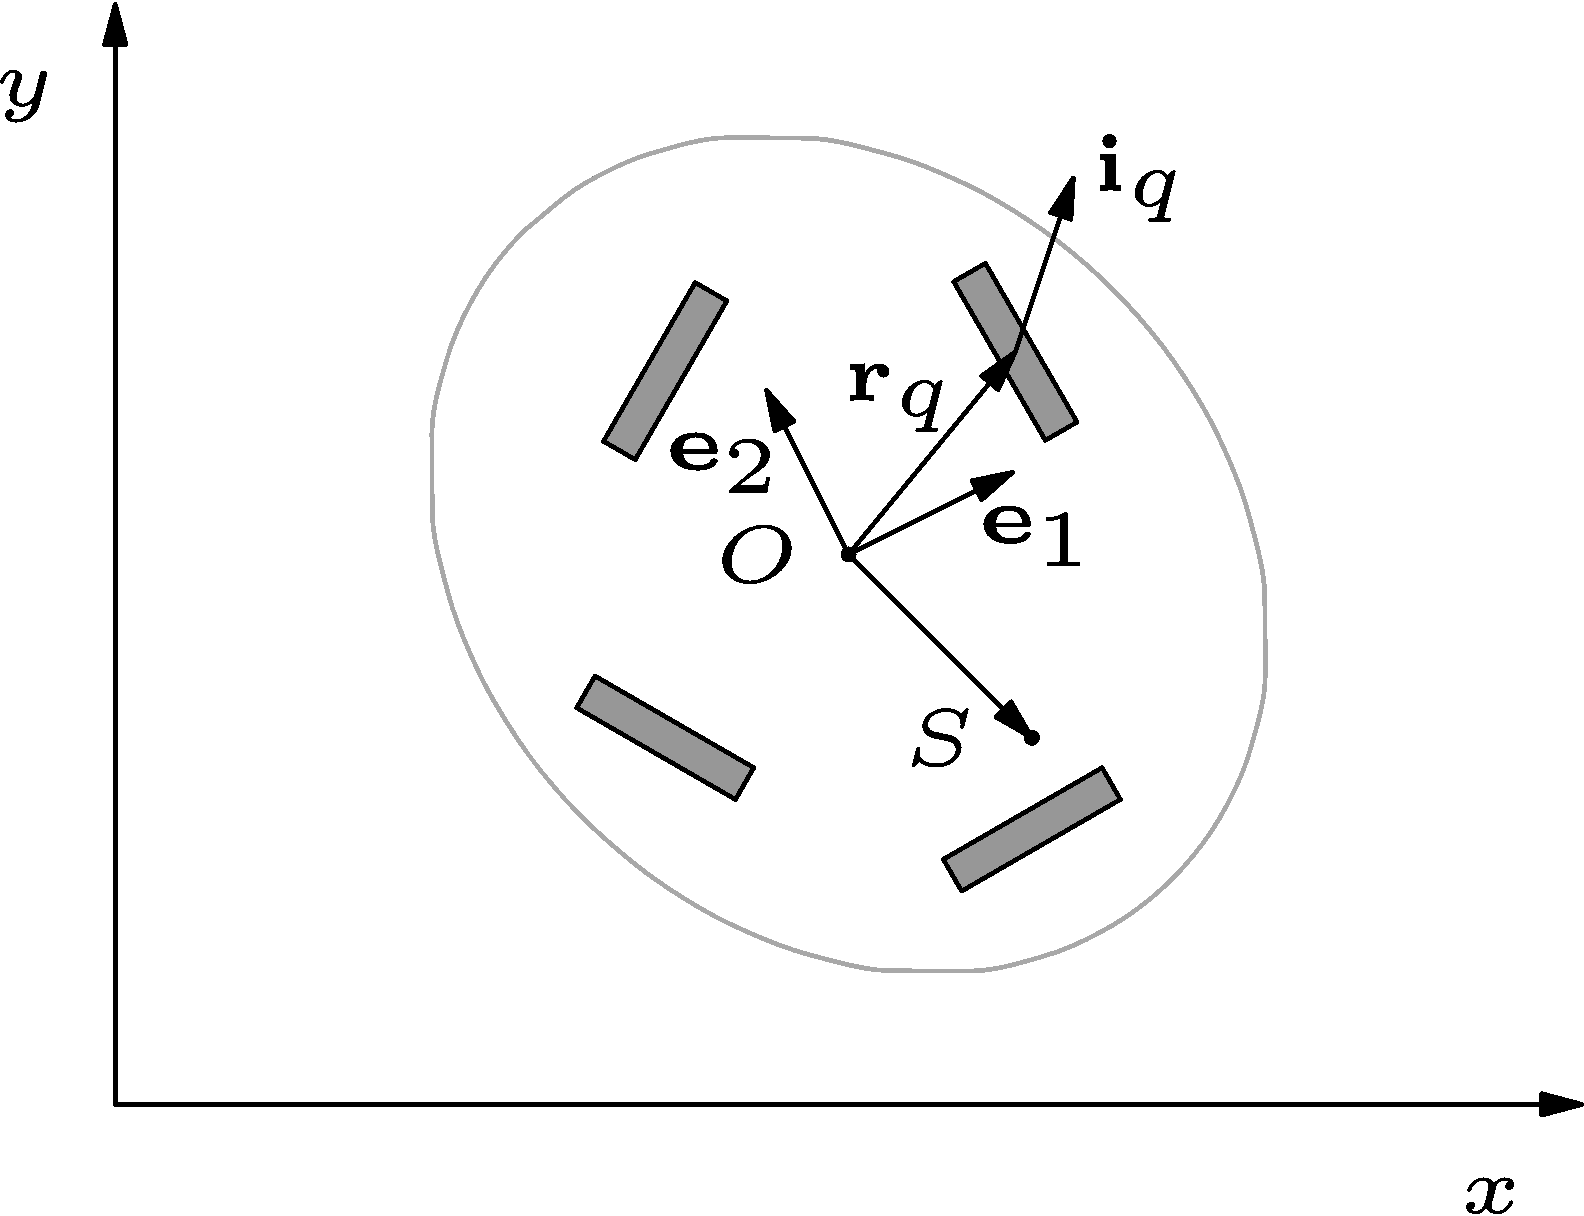
\includegraphics[width=0.75\textwidth]{content/pic/asy/cart_bor.png}
    % \asyinclude[width=0.75\textwidth]{content/pic/asy/cart_bor.asy}
    \caption{Безынерционная модель экипажа}
    \label{fig:bor_vehicle}
\end{figure}

Вводится подвижная система отсчета $O\vec{e}_1\vec{e}_2$, связанная с платформой экипажа. В качестве уравнений движения используются уравнения Феррерса. Уравнения движения по инерции имеют вид:
\begin{eqnarray}\label{eq:bor}
    (\Gamma+mE)\dot{\vec{v}}_O + m\dot{\omega}(J\vec{r}_S+\vec{R}_O)+m\omega J(\vec{v}_O + \omega J\vec{r}_S) = 0,\\
    \hat{I}\dot{\omega} + m(J\vec{r}_S+\vec{R}_O)\cdot\dot{\vec{v}}_O+m\omega\vec{v}_O\cdot\vec{r}_S = 0,\\
    \dot{x} = v_1\cos\theta - v_2\sin\theta, \quad \dot{y} = v_1\sin\theta + v_2\cos\theta, \quad \dot{\theta} = \omega,\\
    \Gamma_{kl} = \sum_q \frac{I_q}{s_q^2 l_q^2}\vec{i}_q^k\vec{i}_q^l, \quad \vec{R}_O = m^{-1}\sum_q \frac{I_q}{s_q^2 l_q^2}(J\vec{r}_q\cdot \vec{i}_q) \vec{i}_q,\\
    \hat{I} = I + \sum_q \frac{I_q}{s_q^2 r_q}(J\vec{r}_q\cdot \vec{i}_q)^2,
\end{eqnarray}
где $\hat{I}$ -- суммарный момент инерции системы относительно вертикальной оси, проходящей через начало $O$ подвижной системы отсчета,\newline
$I$ -- момент инерции платформы относительно той же прямой,\newline
$I_i$ -- моменты инерции колес относительно их диаметров,\newline
$s_q = \cos\psi_q$, \quad $l_q$ -- радиусы колес,\newline
$\vec{r}_q$ -- радиусы-векторы точек закрепления осей колес в подвижной системе отсчета,\newline
$J = \left(\begin{array}{cc}0 & 1\\-1 & 0\end{array}\right)$,
\quad $E$ -- единичная матрица\newline
$x,y,\theta$ -- координаты точки $O$ и угол поворота платформы экипажа вокруг вертикальной оси,\newline
$\vec{v}_O, \omega$ -- вектор скорости точки $O$ и скорость поворота платформы,\newline
$\vec{r}_S$ -- координаты центра масс экипажа в подвижной системе отсчета.

% Данная неголономная модель экипажа также реализована на языке Modelica \cite{ModelicaSpec} как часть упомянутой библиотеки \cite{KosenkoBond}. Таким образом, возможно проведение сравнительного анализа физически-ориентированной и идеализированной моделей и верифкация.

В конфигурации экипажа, рассматриваемой в настоящей работе, центр масс совпадает с началом подвижной системы отсчета $\vec{r}_S = 0$. Кроме того, в силу расположения центров колес в вершинах правильного многоугольника, лежащего в плоскости платформы, а также, поскольку все колеса одинаковы, вектор $\vec{R}_O$ также равен нулю. В этих условиях второе уравнение системы~\ref{eq:bor} принимает вид $\hat{I}\dot{\omega} = 0$, откуда следует первый интеграл $\hat{I}\omega = \const$. Этот интеграл разрушается при учете инерции роликов, как показано в разделе~$\ref{sect:eqs}$.

Количество степеней свободы безынерционной модели экипажа с $N$ колесами равно $3 + N$, что меньше количества степеней свободы моделей, учитывающих инерцию всех $n$ роликов каждого колеса -- $3 + N(n - 1)$ в постановке без проскальзывания либо $3 + N(n + 1)$ в постановке с голономными связями. В силу более простой структуры, безынерционная модель может быть использована для верификации более сложных моделей экипажа с омни-колесами.